\section{Myopic World}

\begin{figure}[h]
        \centering
        \begin{subfigure}[t]{0.3\textwidth}
                \includegraphics[width=\textwidth]{Images/MyoResults/1e4/E/output}
                \caption{Results in the Myopic World using 1e4 samples and entropy based reward
                function. RTBSS is not affected by this parameter.}
                \label{fig:m4e}
        \end{subfigure}%
        ~ %add desired spacing between images, e. g. ~, \quad, \qquad, \hfill etc.
          %(or a blank line to force the subfigure onto a new line)
        \begin{subfigure}[t]{0.3\textwidth}
                \includegraphics[width=\textwidth]{Images/MyoResults/1e5/E/output}
                \caption{Results in the Myopic World using 1e5 samples and entropy based reward
                function.}
                \label{fig:m5e}
        \end{subfigure}
        ~ %add desired spacing between images, e. g. ~, \quad, \qquad, \hfill etc.
          %(or a blank line to force the subfigure onto a new line)
        \begin{subfigure}[t]{0.3\textwidth}
                \includegraphics[width=\textwidth]{Images/MyoResults/1e6/E/output}
                \caption{Results in the Myopic World using 1e6 samples and entropy based reward
                function.}
                \label{fig:m6e}
        \end{subfigure}
        \caption{Pictures of animals}\label{fig:me}
\end{figure}

LOTS OF TEXT; LOTS OF TEXT; LOTS OF TEXT; LOTS OF TEXT; LOTS OF TEXT; LOTS OF TEXT; LOTS OF TEXT; LOTS OF TEXT; LOTS OF TEXT; LOTS OF TEXT; LOTS OF TEXT;

\begin{figure}[h]
        \centering
        \begin{subfigure}[t]{0.3\textwidth}
                \includegraphics[width=\textwidth]{Images/MyoResults/1e4/MB/output}
                \caption{Results in the Myopic World using 1e4 samples and max-of-belief based
                reward function. RTBSS is not affected by this parameter.}
                \label{fig:m4m}
        \end{subfigure}%
        ~ %add desired spacing between images, e. g. ~, \quad, \qquad, \hfill etc.
          %(or a blank line to force the subfigure onto a new line)
        \begin{subfigure}[t]{0.3\textwidth}
                \includegraphics[width=\textwidth]{Images/MyoResults/1e5/MB/output}
                \caption{Results in the Myopic World using 1e4 samples and max-of-belief based
                reward function.}
                \label{fig:m5m}
        \end{subfigure}
        ~ %add desired spacing between images, e. g. ~, \quad, \qquad, \hfill etc.
          %(or a blank line to force the subfigure onto a new line)
        \begin{subfigure}[t]{0.3\textwidth}
                \includegraphics[width=\textwidth]{Images/MyoResults/1e6/MB/output}
                \caption{Results in the Myopic World using 1e4 samples and max-of-belief based
                reward function.}
                \label{fig:m6m}
        \end{subfigure}
        \caption{Pictures of animals}\label{fig:mm}
\end{figure}

\clearpage
\section{Finite Budget}

\begin{figure}[h]
        \centering
        \begin{subfigure}[t]{0.3\textwidth}
                \includegraphics[width=\textwidth]{Images/FiniteBudgetResults/0.5/1e4/E/output}
                \caption{Results in the Finite Budget World using 1e4 samples and entropy based reward
                function. RTBSS is not affected by this parameter.}
                \label{fig:m4e}
        \end{subfigure}%
        ~ %add desired spacing between images, e. g. ~, \quad, \qquad, \hfill etc.
          %(or a blank line to force the subfigure onto a new line)
        \begin{subfigure}[t]{0.3\textwidth}
                \includegraphics[width=\textwidth]{Images/FiniteBudgetResults/0.5/1e5/E/output}
                \caption{Results in the Finite Budget World using 1e5 samples and entropy based reward
                function.}
                \label{fig:m5e}
        \end{subfigure}
        ~ %add desired spacing between images, e. g. ~, \quad, \qquad, \hfill etc.
          %(or a blank line to force the subfigure onto a new line)
        \begin{subfigure}[t]{0.3\textwidth}
                \includegraphics[width=\textwidth]{Images/FiniteBudgetResults/0.5/1e6/E/output}
                \caption{Results in the Finite Budget World using 1e6 samples and entropy based reward
                function.}
                \label{fig:m6e}
        \end{subfigure}
        \caption{Pictures of animals}\label{fig:me}
\end{figure}

LOTS OF TEXT; LOTS OF TEXT; LOTS OF TEXT; LOTS OF TEXT; LOTS OF TEXT; LOTS OF TEXT; LOTS OF TEXT; LOTS OF TEXT; LOTS OF TEXT; LOTS OF TEXT; LOTS OF TEXT;

\begin{figure}[h]
        \centering
        \begin{subfigure}[t]{0.3\textwidth}
                \includegraphics[width=\textwidth]{Images/FiniteBudgetResults/0.5/1e4/MB/output}
                \caption{Results in the Finite Budget World using 1e4 samples and max-of-belief based
                reward function. RTBSS is not affected by this parameter.}
                \label{fig:m4m}
        \end{subfigure}%
        ~ %add desired spacing between images, e. g. ~, \quad, \qquad, \hfill etc.
          %(or a blank line to force the subfigure onto a new line)
        \begin{subfigure}[t]{0.3\textwidth}
                \includegraphics[width=\textwidth]{Images/FiniteBudgetResults/0.5/1e5/MB/output}
                \caption{Results in the Finite Budget World using 1e4 samples and max-of-belief based
                reward function.}
                \label{fig:m5m}
        \end{subfigure}
        ~ %add desired spacing between images, e. g. ~, \quad, \qquad, \hfill etc.
          %(or a blank line to force the subfigure onto a new line)
        \begin{subfigure}[t]{0.3\textwidth}
                \includegraphics[width=\textwidth]{Images/FiniteBudgetResults/0.5/1e6/MB/output}
                \caption{Results in the Finite Budget World using 1e4 samples and max-of-belief based
                reward function.}
                \label{fig:m6m}
        \end{subfigure}
        \caption{Pictures of animals}\label{fig:mm}
\end{figure}

\begin{figure}[h]
        \centering
        \begin{subfigure}[t]{0.3\textwidth}
                \includegraphics[width=\textwidth]{Images/FiniteBudgetResults/0.75/1e4/E/output}
                \caption{Results in the Finite Budget World using 1e4 samples and entropy based reward
                function. RTBSS is not affected by this parameter.}
                \label{fig:m4e}
        \end{subfigure}%
        ~ %add desired spacing between images, e. g. ~, \quad, \qquad, \hfill etc.
          %(or a blank line to force the subfigure onto a new line)
        \begin{subfigure}[t]{0.3\textwidth}
                \includegraphics[width=\textwidth]{Images/FiniteBudgetResults/0.75/1e5/E/output}
                \caption{Results in the Finite Budget World using 1e5 samples and entropy based reward
                function.}
                \label{fig:m5e}
        \end{subfigure}
        ~ %add desired spacing between images, e. g. ~, \quad, \qquad, \hfill etc.
          %(or a blank line to force the subfigure onto a new line)
        \begin{subfigure}[t]{0.3\textwidth}
                \includegraphics[width=\textwidth]{Images/FiniteBudgetResults/0.75/1e6/E/output}
                \caption{Results in the Finite Budget World using 1e6 samples and entropy based reward
                function.}
                \label{fig:m6e}
        \end{subfigure}
        \caption{Pictures of animals}\label{fig:me}
\end{figure}

LOTS OF TEXT; LOTS OF TEXT; LOTS OF TEXT; LOTS OF TEXT; LOTS OF TEXT; LOTS OF TEXT; LOTS OF TEXT; LOTS OF TEXT; LOTS OF TEXT; LOTS OF TEXT; LOTS OF TEXT;

\begin{figure}[h]
        \centering
        \begin{subfigure}[t]{0.3\textwidth}
                \includegraphics[width=\textwidth]{Images/FiniteBudgetResults/0.75/1e4/MB/output}
                \caption{Results in the Finite Budget World using 1e4 samples and max-of-belief based
                reward function. RTBSS is not affected by this parameter.}
                \label{fig:m4m}
        \end{subfigure}%
        ~ %add desired spacing between images, e. g. ~, \quad, \qquad, \hfill etc.
          %(or a blank line to force the subfigure onto a new line)
        \begin{subfigure}[t]{0.3\textwidth}
                \includegraphics[width=\textwidth]{Images/FiniteBudgetResults/0.75/1e5/MB/output}
                \caption{Results in the Finite Budget World using 1e4 samples and max-of-belief based
                reward function.}
                \label{fig:m5m}
        \end{subfigure}
        ~ %add desired spacing between images, e. g. ~, \quad, \qquad, \hfill etc.
          %(or a blank line to force the subfigure onto a new line)
        \begin{subfigure}[t]{0.3\textwidth}
                \includegraphics[width=\textwidth]{Images/FiniteBudgetResults/0.75/1e6/MB/output}
                \caption{Results in the Finite Budget World using 1e4 samples and max-of-belief based
                reward function.}
                \label{fig:m6m}
        \end{subfigure}
        \caption{Pictures of animals}\label{fig:mm}
\end{figure}

\clearpage
\section{Camera World}

\begin{figure}[h]
        \centering
        \begin{subfigure}[t]{0.3\textwidth}
                \includegraphics[width=\textwidth]{Images/CameraBasicResults/Small_20x20/1e4/E/output}
                \caption{Results in the Camera World using 1e4 samples and entropy based reward
                function. RTBSS is not affected by this parameter.}
                \label{fig:m4e}
        \end{subfigure}%
        ~ %add desired spacing between images, e. g. ~, \quad, \qquad, \hfill etc.
          %(or a blank line to force the subfigure onto a new line)
        \begin{subfigure}[t]{0.3\textwidth}
                \includegraphics[width=\textwidth]{Images/CameraBasicResults/Small_20x20/1e6/E/output}
                \caption{Results in the Camera World using 1e5 samples and entropy based reward
                function.}
                \label{fig:m5e}
        \end{subfigure}
        ~ %add desired spacing between images, e. g. ~, \quad, \qquad, \hfill etc.
          %(or a blank line to force the subfigure onto a new line)
        \begin{subfigure}[t]{0.3\textwidth}
                \includegraphics[width=\textwidth]{Images/CameraBasicResults/Small_20x20/1e6/E/output}
                \caption{Results in the Camera World using 1e6 samples and entropy based reward
                function.}
                \label{fig:m6e}
        \end{subfigure}
        \caption{Pictures of animals}\label{fig:me}
\end{figure}

\begin{figure}[h]
        \centering
        \begin{subfigure}[t]{0.3\textwidth}
                \includegraphics[width=\textwidth]{Images/CameraBasicResults/Small_20x20/1e4/MB/output}
                \caption{Results in the Camera World using 1e4 samples and entropy based reward
                function. RTBSS is not affected by this parameter.}
                \label{fig:m4e}
        \end{subfigure}%
        ~ %add desired spacing between images, e. g. ~, \quad, \qquad, \hfill etc.
          %(or a blank line to force the subfigure onto a new line)
        \begin{subfigure}[t]{0.3\textwidth}
                \includegraphics[width=\textwidth]{Images/CameraBasicResults/Small_20x20/1e6/MB/output}
                \caption{Results in the Camera World using 1e5 samples and entropy based reward
                function.}
                \label{fig:m5e}
        \end{subfigure}
        ~ %add desired spacing between images, e. g. ~, \quad, \qquad, \hfill etc.
          %(or a blank line to force the subfigure onto a new line)
        \begin{subfigure}[t]{0.3\textwidth}
                \includegraphics[width=\textwidth]{Images/CameraBasicResults/Small_20x20/1e6/MB/output}
                \caption{Results in the Camera World using 1e6 samples and entropy based reward
                function.}
                \label{fig:m6e}
        \end{subfigure}
        \caption{Pictures of animals}\label{fig:me}
\end{figure}

\begin{figure}[h]
        \centering
        \begin{subfigure}[t]{0.3\textwidth}
                \includegraphics[width=\textwidth]{Images/CameraBasicResults/Big_50x50/1e4/E/output}
                \caption{Results in the Camera World using 1e4 samples and entropy based reward
                function. RTBSS is not affected by this parameter.}
                \label{fig:m4e}
        \end{subfigure}%
        ~ %add desired spacing between images, e. g. ~, \quad, \qquad, \hfill etc.
          %(or a blank line to force the subfigure onto a new line)
        \begin{subfigure}[t]{0.3\textwidth}
                \includegraphics[width=\textwidth]{Images/CameraBasicResults/Big_50x50/1e6/E/output}
                \caption{Results in the Camera World using 1e5 samples and entropy based reward
                function.}
                \label{fig:m5e}
        \end{subfigure}
        ~ %add desired spacing between images, e. g. ~, \quad, \qquad, \hfill etc.
          %(or a blank line to force the subfigure onto a new line)
        \begin{subfigure}[t]{0.3\textwidth}
                \includegraphics[width=\textwidth]{Images/CameraBasicResults/Big_50x50/1e6/E/output}
                \caption{Results in the Camera World using 1e6 samples and entropy based reward
                function.}
                \label{fig:m6e}
        \end{subfigure}
        \caption{Pictures of animals}\label{fig:me}
\end{figure}

\begin{figure}[h]
        \centering
        \begin{subfigure}[t]{0.3\textwidth}
                \includegraphics[width=\textwidth]{Images/CameraBasicResults/Big_50x50/1e4/MB/output}
                \caption{Results in the Camera World using 1e4 samples and entropy based reward
                function. RTBSS is not affected by this parameter.}
                \label{fig:m4e}
        \end{subfigure}%
        ~ %add desired spacing between images, e. g. ~, \quad, \qquad, \hfill etc.
          %(or a blank line to force the subfigure onto a new line)
        \begin{subfigure}[t]{0.3\textwidth}
                \includegraphics[width=\textwidth]{Images/CameraBasicResults/Big_50x50/1e6/MB/output}
                \caption{Results in the Camera World using 1e5 samples and entropy based reward
                function.}
                \label{fig:m5e}
        \end{subfigure}
        ~ %add desired spacing between images, e. g. ~, \quad, \qquad, \hfill etc.
          %(or a blank line to force the subfigure onto a new line)
        \begin{subfigure}[t]{0.3\textwidth}
                \includegraphics[width=\textwidth]{Images/CameraBasicResults/Big_50x50/1e6/MB/output}
                \caption{Results in the Camera World using 1e6 samples and entropy based reward
                function.}
                \label{fig:m6e}
        \end{subfigure}
        \caption{Pictures of animals}\label{fig:me}
\end{figure}

\begin{figure}[h]
        \centering
        \begin{subfigure}[t]{0.5\textwidth}
                \includegraphics[width=\textwidth]{Images/CameraBasicResults/Big_50x50/Multi/E/output}
                \caption{Results in the Camera World using 1e4 samples and entropy based reward
                function. RTBSS is not affected by this parameter.}
                \label{fig:m4e}
        \end{subfigure}%
        ~ %add desired spacing between images, e. g. ~, \quad, \qquad, \hfill etc.
          %(or a blank line to force the subfigure onto a new line)
        \begin{subfigure}[t]{0.5\textwidth}
                \includegraphics[width=\textwidth]{Images/CameraBasicResults/Big_50x50/Multi/MB/output}
                \caption{Results in the Camera World using 1e5 samples and entropy based reward
                function.}
                \label{fig:m5e}
        \end{subfigure}
        \caption{Pictures of animals}\label{fig:me}
\end{figure}

\begin{figure}[h]
        \centering
        \begin{subfigure}[t]{0.3\textwidth}
                \includegraphics[width=\textwidth]{Images/CameraPathResults/Small_20x20/1e4/E/output}
                \caption{Results in the Camera World using 1e4 samples and entropy based reward
                function. RTBSS is not affected by this parameter.}
                \label{fig:m4e}
        \end{subfigure}%
        ~ %add desired spacing between images, e. g. ~, \quad, \qquad, \hfill etc.
          %(or a blank line to force the subfigure onto a new line)
        \begin{subfigure}[t]{0.3\textwidth}
                \includegraphics[width=\textwidth]{Images/CameraPathResults/Small_20x20/1e6/E/output}
                \caption{Results in the Camera World using 1e5 samples and entropy based reward
                function.}
                \label{fig:m5e}
        \end{subfigure}
        ~ %add desired spacing between images, e. g. ~, \quad, \qquad, \hfill etc.
          %(or a blank line to force the subfigure onto a new line)
        \begin{subfigure}[t]{0.3\textwidth}
                \includegraphics[width=\textwidth]{Images/CameraPathResults/Small_20x20/1e6/E/output}
                \caption{Results in the Camera World using 1e6 samples and entropy based reward
                function.}
                \label{fig:m6e}
        \end{subfigure}
        \caption{Pictures of animals}\label{fig:me}
\end{figure}

\begin{figure}[h]
        \centering
        \begin{subfigure}[t]{0.3\textwidth}
                \includegraphics[width=\textwidth]{Images/CameraPathResults/Small_20x20/1e4/MB/output}
                \caption{Results in the Camera World using 1e4 samples and entropy based reward
                function. RTBSS is not affected by this parameter.}
                \label{fig:m4e}
        \end{subfigure}%
        ~ %add desired spacing between images, e. g. ~, \quad, \qquad, \hfill etc.
          %(or a blank line to force the subfigure onto a new line)
        \begin{subfigure}[t]{0.3\textwidth}
                \includegraphics[width=\textwidth]{Images/CameraPathResults/Small_20x20/1e6/MB/output}
                \caption{Results in the Camera World using 1e5 samples and entropy based reward
                function.}
                \label{fig:m5e}
        \end{subfigure}
        ~ %add desired spacing between images, e. g. ~, \quad, \qquad, \hfill etc.
          %(or a blank line to force the subfigure onto a new line)
        \begin{subfigure}[t]{0.3\textwidth}
                \includegraphics[width=\textwidth]{Images/CameraPathResults/Small_20x20/1e6/MB/output}
                \caption{Results in the Camera World using 1e6 samples and entropy based reward
                function.}
                \label{fig:m6e}
        \end{subfigure}
        \caption{Pictures of animals}\label{fig:me}
\end{figure}

\begin{figure}[h]
        \centering
        \begin{subfigure}[t]{0.3\textwidth}
                \includegraphics[width=\textwidth]{Images/CameraPathResults/Big_50x50/1e4/E/output}
                \caption{Results in the Camera World using 1e4 samples and entropy based reward
                function. RTBSS is not affected by this parameter.}
                \label{fig:m4e}
        \end{subfigure}%
        ~ %add desired spacing between images, e. g. ~, \quad, \qquad, \hfill etc.
          %(or a blank line to force the subfigure onto a new line)
        \begin{subfigure}[t]{0.3\textwidth}
                \includegraphics[width=\textwidth]{Images/CameraPathResults/Big_50x50/1e6/E/output}
                \caption{Results in the Camera World using 1e5 samples and entropy based reward
                function.}
                \label{fig:m5e}
        \end{subfigure}
        ~ %add desired spacing between images, e. g. ~, \quad, \qquad, \hfill etc.
          %(or a blank line to force the subfigure onto a new line)
        \begin{subfigure}[t]{0.3\textwidth}
                \includegraphics[width=\textwidth]{Images/CameraPathResults/Big_50x50/1e6/E/output}
                \caption{Results in the Camera World using 1e6 samples and entropy based reward
                function.}
                \label{fig:m6e}
        \end{subfigure}
        \caption{Pictures of animals}\label{fig:me}
\end{figure}

\begin{figure}[h]
        \centering
        \begin{subfigure}[t]{0.3\textwidth}
                \includegraphics[width=\textwidth]{Images/CameraPathResults/Big_50x50/1e4/MB/output}
                \caption{Results in the Camera World using 1e4 samples and entropy based reward
                function. RTBSS is not affected by this parameter.}
                \label{fig:m4e}
        \end{subfigure}%
        ~ %add desired spacing between images, e. g. ~, \quad, \qquad, \hfill etc.
          %(or a blank line to force the subfigure onto a new line)
        \begin{subfigure}[t]{0.3\textwidth}
                \includegraphics[width=\textwidth]{Images/CameraPathResults/Big_50x50/1e6/MB/output}
                \caption{Results in the Camera World using 1e5 samples and entropy based reward
                function.}
                \label{fig:m5e}
        \end{subfigure}
        ~ %add desired spacing between images, e. g. ~, \quad, \qquad, \hfill etc.
          %(or a blank line to force the subfigure onto a new line)
        \begin{subfigure}[t]{0.3\textwidth}
                \includegraphics[width=\textwidth]{Images/CameraPathResults/Big_50x50/1e6/MB/output}
                \caption{Results in the Camera World using 1e6 samples and entropy based reward
                function.}
                \label{fig:m6e}
        \end{subfigure}
        \caption{Pictures of animals}\label{fig:me}
\end{figure}

\begin{figure}[h]
        \centering
        \begin{subfigure}[t]{0.5\textwidth}
                \includegraphics[width=\textwidth]{Images/CameraPathResults/Big_50x50/Multi/E/output}
                \caption{Results in the Camera World using 1e4 samples and entropy based reward
                function. RTBSS is not affected by this parameter.}
                \label{fig:m4e}
        \end{subfigure}%
        ~ %add desired spacing between images, e. g. ~, \quad, \qquad, \hfill etc.
          %(or a blank line to force the subfigure onto a new line)
        \begin{subfigure}[t]{0.5\textwidth}
                \includegraphics[width=\textwidth]{Images/CameraPathResults/Big_50x50/Multi/MB/output}
                \caption{Results in the Camera World using 1e5 samples and entropy based reward
                function.}
                \label{fig:m5e}
        \end{subfigure}
        \caption{Pictures of animals}\label{fig:me}
\end{figure}
